\section{Results}
\label{sec:results}

\para{Data audit.}
\tabref{tab:data_audit} reports the oracle sizes and label prevalence. The \mpdata pool has high stable or \nearhull prevalence at 56.80\%, so random search is a strong baseline rather than a sparse-discovery lower bound. The \gnome transfer set is even more enriched, with 86.96\% on-hull candidates and 98.41\% near-hull candidates by the thresholds used here.

\begin{table}[t]
    \centering
    \caption{Dataset audit for the offline discovery benchmark. Stable or \nearhull means energy above hull $\leq 0.05$ eV/atom for \mpdata. On-hull for \gnome means decomposition energy per atom $\leq 0.0$.}
    \label{tab:data_audit}
    \begin{tabular}{@{}lr@{}}
        \toprule
        Quantity & Value \\
        \midrule
        \mpdata raw rows & 133,420 \\
        \mpdata labeled rows used & 129,622 \\
        Missing energy-above-hull rows excluded & 3,798 \\
        Stable or \nearhull rows & 73,630 \\
        Stable prevalence & 56.80\% \\
        \gnome R2SCAN rows & 139,541 \\
        \gnome on-hull prevalence & 86.96\% \\
        \gnome near-hull prevalence & 98.41\% \\
        \bottomrule
    \end{tabular}
\end{table}


\para{The surrogate learns useful stability signal.}
\tabref{tab:predictive_signal} and \figref{fig:predictive_signal} show held-out predictive performance. Composition-only descriptors reach ROC-AUC 0.846 and average precision 0.865. Adding coarse cell descriptors improves ROC-AUC to 0.874, average precision to 0.891, and F1 to 0.828. This supports the first hypothesis: simple leakage-controlled descriptors contain enough signal to rank stable and \nearhull candidates.

\begin{table}[t]
    \centering
    \caption{Held-out predictive signal for the stability surrogate. Higher is better for all metrics. Best results in {\bf bold}.}
    \label{tab:predictive_signal}
    \begin{tabular}{@{}lccccc@{}}
        \toprule
        Feature set & ROC-AUC & Avg. precision & F1 & Precision & Recall \\
        \midrule
        Composition only & 0.846 & 0.865 & 0.809 & 0.756 & 0.871 \\
        Composition plus cell & {\bf 0.874} & {\bf 0.891} & {\bf 0.828} & {\bf 0.779} & {\bf 0.883} \\
        \bottomrule
    \end{tabular}
\end{table}


\begin{figure}[t]
    \centering
    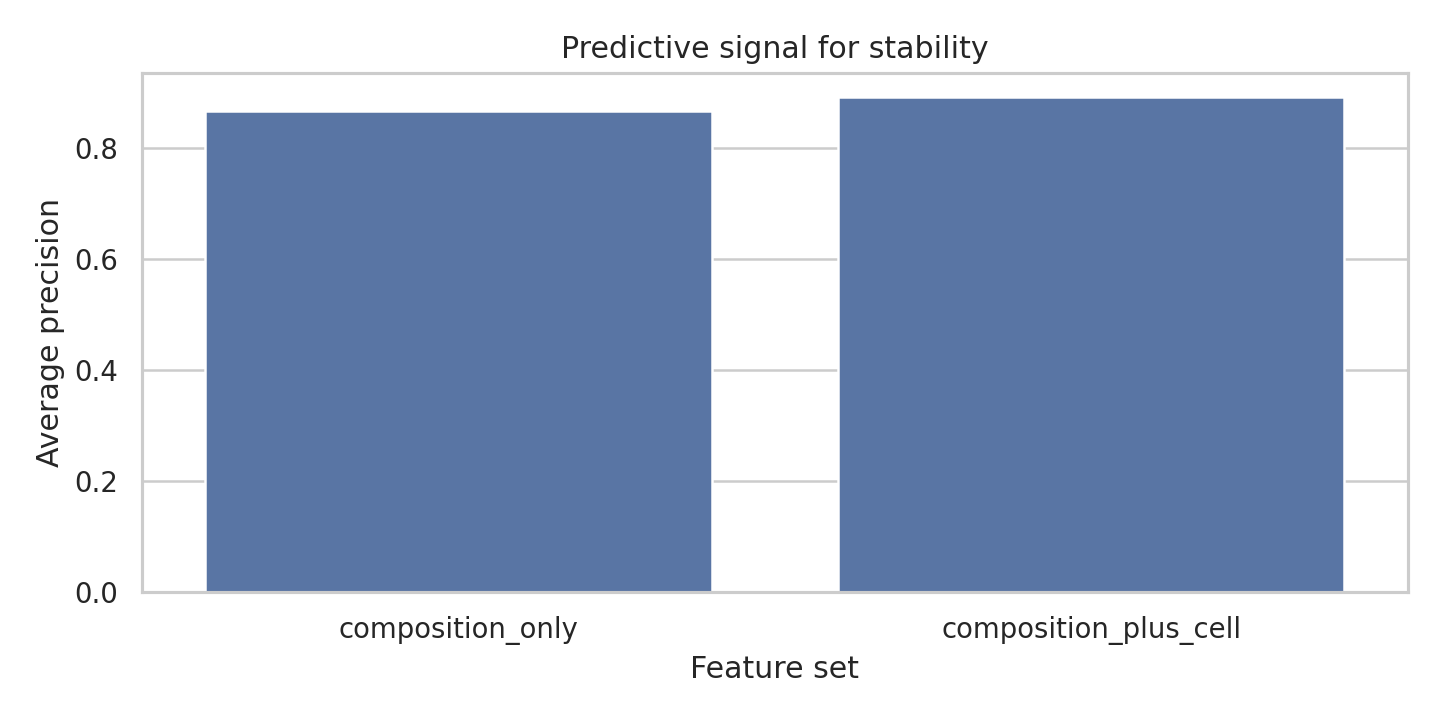
\includegraphics[width=0.90\linewidth]{figures/predictive_signal.png}
    \caption{Predictive signal from leakage-controlled descriptors. The composition-plus-cell feature set improves the ROC and precision-recall behavior over composition-only features, showing that the surrogate has useful ranking signal before it is used inside the active-discovery loop.}
    \label{fig:predictive_signal}
\end{figure}

\para{Model-guided policies discover many more stable candidates than random.}
\tabref{tab:active_summary} reports final performance after 2,400 validations. \diverseucb finds the most stable candidates on average: 1,933.2 compared with 1,364.8 for random. Greedy and standard \ucb are close behind, with 1,922.6 and 1,904.8 stable discoveries. All three reward-oriented policies increase stable precision from 0.5687 for random to 0.7937--0.8055. \figref{fig:active_discovery} shows that these gains accumulate across acquisition rounds rather than appearing only at the final budget.

\begin{table}[t]
    \centering
    \caption{Final active-discovery performance at a fixed 2,400-candidate validation budget. Higher is better for all metrics. Best results in {\bf bold}.}
    \label{tab:active_summary}
    \begin{tabular}{@{}lrrrr@{}}
        \toprule
        Policy & Mean stable found & Mean precision & Mean acceleration & Mean recall \\
        \midrule
        \diverseucb & {\bf 1,933.2} & {\bf 0.8055} & {\bf 1.4186} & {\bf 0.1362} \\
        Greedy & 1,922.6 & 0.8011 & 1.4108 & 0.1354 \\
        \ucb & 1,904.8 & 0.7937 & 1.3977 & 0.1342 \\
        Random & 1,364.8 & 0.5687 & 1.0015 & 0.0961 \\
        Uncertainty & 1,286.6 & 0.5361 & 0.9442 & 0.0906 \\
        \bottomrule
    \end{tabular}
\end{table}


\begin{figure}[t]
    \centering
    \begin{subfigure}[b]{0.49\textwidth}
        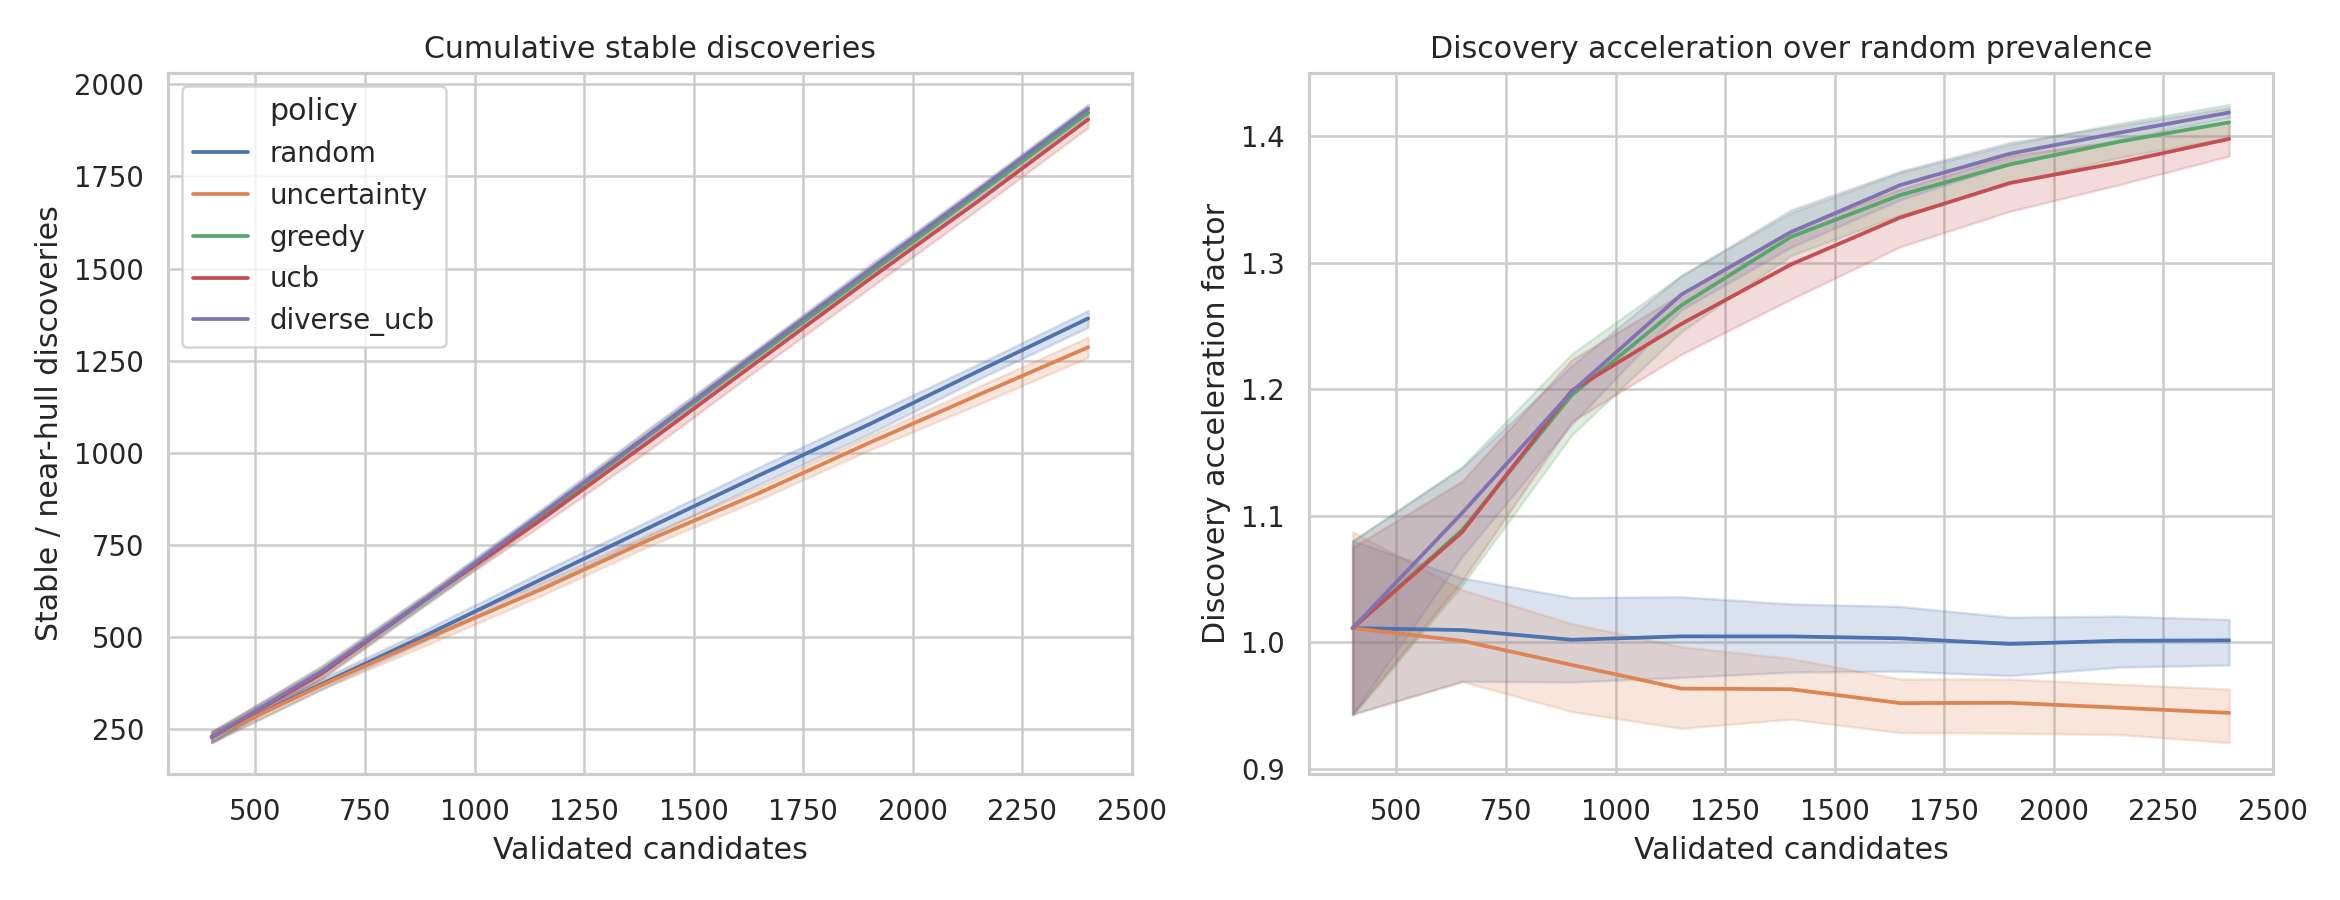
\includegraphics[width=\textwidth]{figures/active_learning_curves.png}
        \caption{Discovery traces}
        \label{fig:active_curves}
    \end{subfigure}
    \hfill
    \begin{subfigure}[b]{0.49\textwidth}
        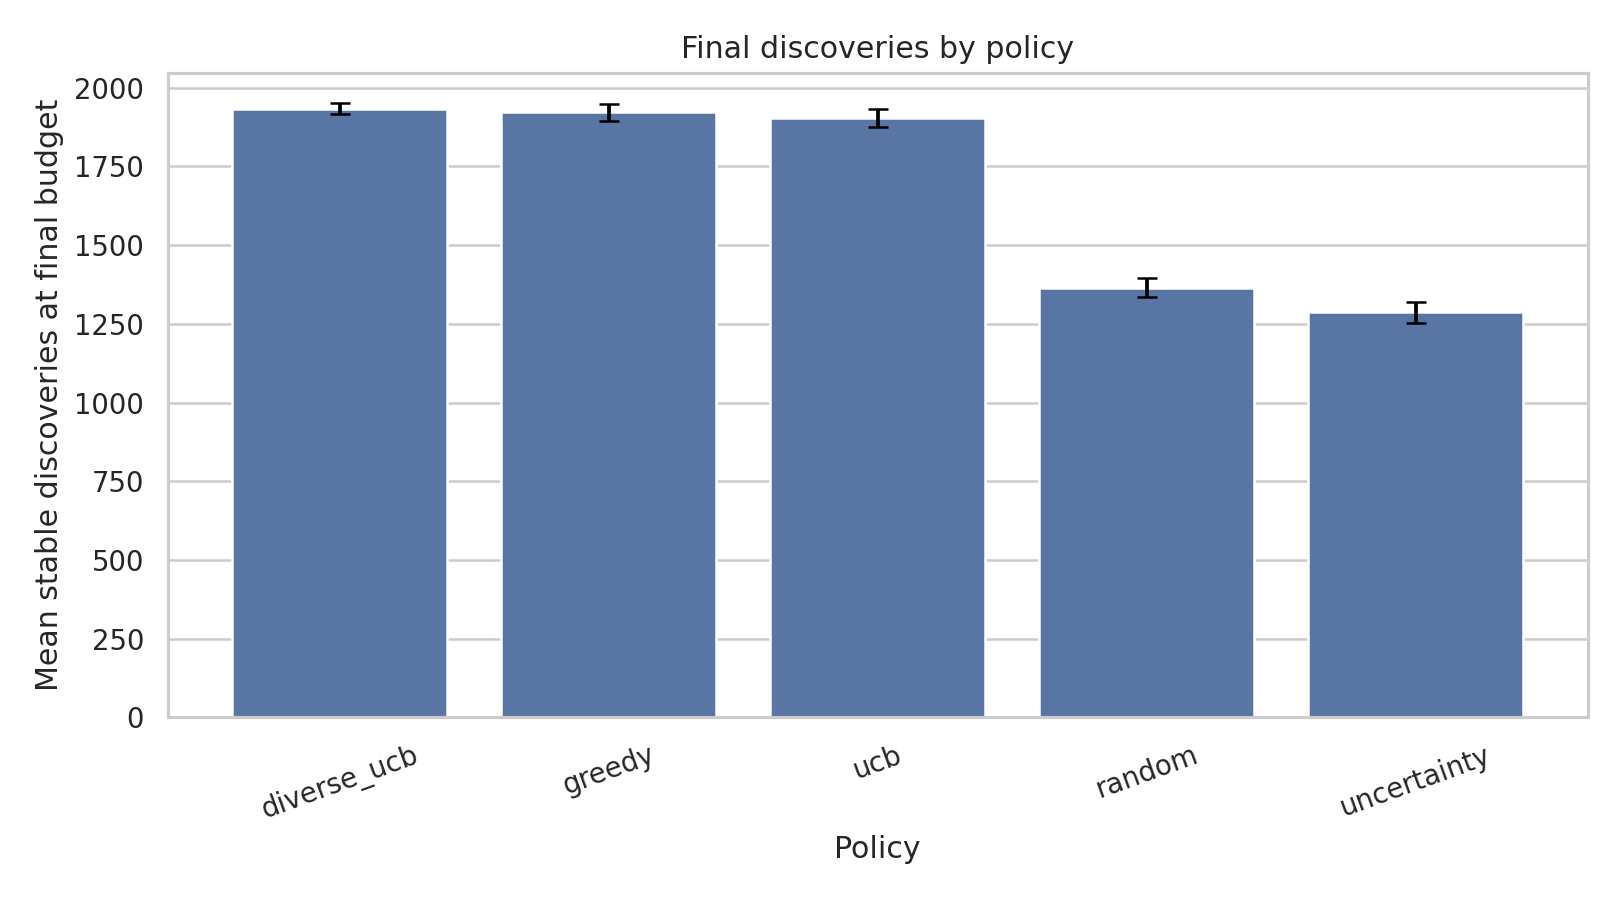
\includegraphics[width=\textwidth]{figures/active_final_discoveries.png}
        \caption{Final discoveries}
        \label{fig:active_final}
    \end{subfigure}
    \caption{Budgeted active discovery on \mpdata. Reward-oriented policies dominate random selection under the same validation budget. Uncertainty sampling underperforms random, which shows that selecting ambiguous examples is not the same as selecting high-value candidates.}
    \label{fig:active_discovery}
\end{figure}

\para{The gains are statistically large across matched seeds.}
\tabref{tab:stat_tests} gives paired tests against random. \diverseucb improves final stable discoveries by +568.4 candidates with a 95\% confidence interval of [524.0, 612.8] and Holm-adjusted $p=1.05 \times 10^{-5}$. Greedy improves by +557.8 and \ucb by +540.0. Uncertainty sampling is significantly worse than random by -78.2 discoveries, with Holm-adjusted $p=0.0136$. The main positive result is therefore not just ``learning helps''; it is that reward-oriented acquisition is necessary.

\begin{table}[t]
    \centering
    \caption{Paired policy comparisons against random across five matched seeds. Confidence intervals are for final stable-discovery differences.}
    \label{tab:stat_tests}
    \resizebox{\textwidth}{!}{%
    \begin{tabular}{@{}lrrrr@{}}
        \toprule
        Comparison & Mean difference & 95\% CI & Cohen's $d$ & Holm-adjusted $p$ \\
        \midrule
        \diverseucb vs. random & {\bf +568.4} & [524.0, 612.8] & 15.90 & $1.05 \times 10^{-5}$ \\
        Greedy vs. random & +557.8 & [514.9, 600.7] & 16.16 & $1.05 \times 10^{-5}$ \\
        \ucb vs. random & +540.0 & [515.3, 564.7] & {\bf 27.19} & {\bf $1.75 \times 10^{-6}$} \\
        Uncertainty vs. random & -78.2 & [-129.8, -26.6] & -1.88 & 0.0136 \\
        \bottomrule
    \end{tabular}
    }
\end{table}


\para{External transfer is positive but modest.}
We apply the composition-only \mpdata model to \gnome R2SCAN summaries because full structures were not locally mirrored. \tabref{tab:gnome_transfer} and \figref{fig:gnome_transfer} show that the top-ranked 100 candidates have a 0.970 on-hull rate compared with 0.8735 for random samples, an on-hull acceleration of 1.115. The gains remain positive through the top 10,000 but are modest because the \gnome set is already highly enriched.

\begin{table}[t]
    \centering
    \caption{\gnome transfer ranking with the composition-only \mpdata surrogate. Top-ranked candidates improve on-hull enrichment over random samples, while near-hull rates are nearly saturated.}
    \label{tab:gnome_transfer}
    \begin{tabular}{@{}rrrr@{}}
        \toprule
        Top $K$ & Top on-hull rate & Random on-hull rate & On-hull acceleration \\
        \midrule
        100 & {\bf 0.970} & 0.8735 & {\bf 1.115} \\
        500 & 0.920 & 0.8691 & 1.058 \\
        1,000 & 0.917 & 0.8702 & 1.055 \\
        5,000 & 0.937 & 0.8697 & 1.078 \\
        10,000 & 0.929 & 0.8697 & 1.068 \\
        \bottomrule
    \end{tabular}
\end{table}


\begin{figure}[t]
    \centering
    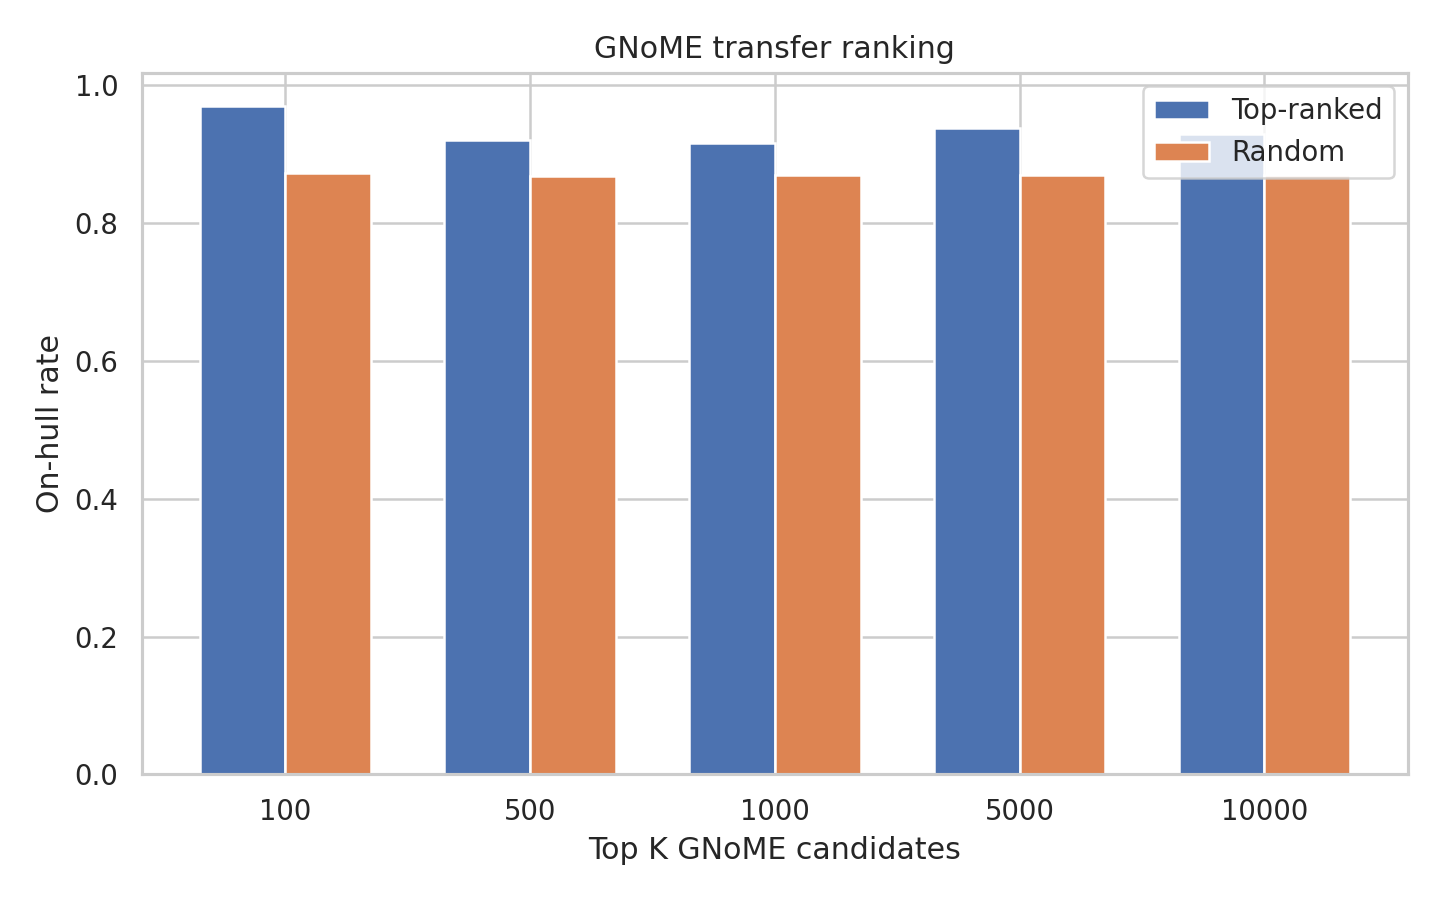
\includegraphics[width=0.86\linewidth]{figures/gnome_transfer_topk.png}
    \caption{\gnome transfer ranking. A composition-only surrogate trained on \mpdata improves on-hull enrichment in the top-ranked \gnome candidates, especially at top 100. Near-hull rates are close to saturated, so the stricter on-hull rate is the more informative transfer metric.}
    \label{fig:gnome_transfer}
\end{figure}

\para{The run is reproducible under a deterministic mini-rerun.}
The experiment included a same-seed repeat of the greedy policy. Both runs produced identical traces for seed 13, with \texttt{same\_trace=true}. This check does not prove full cross-platform determinism, but it confirms that the recorded run artifacts are internally reproducible in the configured environment.
